% Created 2022-01-31 Mon 18:45
% Intended LaTeX compiler: pdflatex
\documentclass[11pt]{article}
\usepackage[utf8]{inputenc}
\usepackage[T1]{fontenc}
\usepackage{graphicx}
\usepackage{longtable}
\usepackage{wrapfig}
\usepackage{rotating}
\usepackage[normalem]{ulem}
\usepackage{amsmath}
\usepackage{amssymb}
\usepackage{capt-of}
\usepackage{hyperref}
\usepackage{color}
\usepackage{listings}
\usepackage{color}
\usepackage{listings}
\author{Maikol Solís}
\date{\textit{<2022-02-01 Tue>}}
\title{Emacs workshop 2022: Day 5}
\hypersetup{
 pdfauthor={Maikol Solís},
 pdftitle={Emacs workshop 2022: Day 5},
 pdfkeywords={},
 pdfsubject={},
 pdfcreator={Emacs 27.2 (Org mode 9.6)}, 
 pdflang={English}}
\usepackage{biblatex}

\begin{document}


\section{Git basics}
\label{sec:orgef41def}

\subsection{Why git is important?}
\label{sec:org94decb8}

\begin{center}

\includegraphics[width=.9\linewidth]{./final.jpg}
\end{center}

\newpage
\subsection{What is git?}
\label{sec:orgdc7b64a}

Git is a Version Control System (VCS) that is designed to track files and changes among multiple users.

\begin{center}
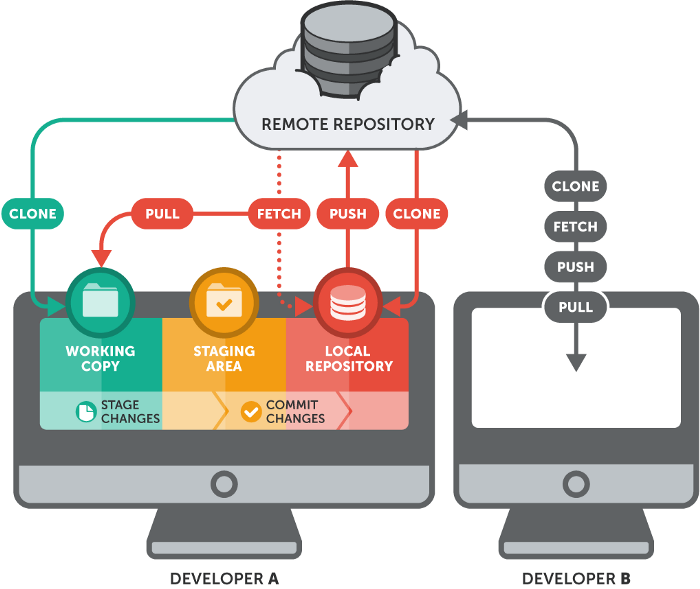
\includegraphics[width=.9\linewidth]{./remote.png}
\end{center}

\newpage
\subsection{How does it work?}
\label{sec:org3adb940}



\begin{center}
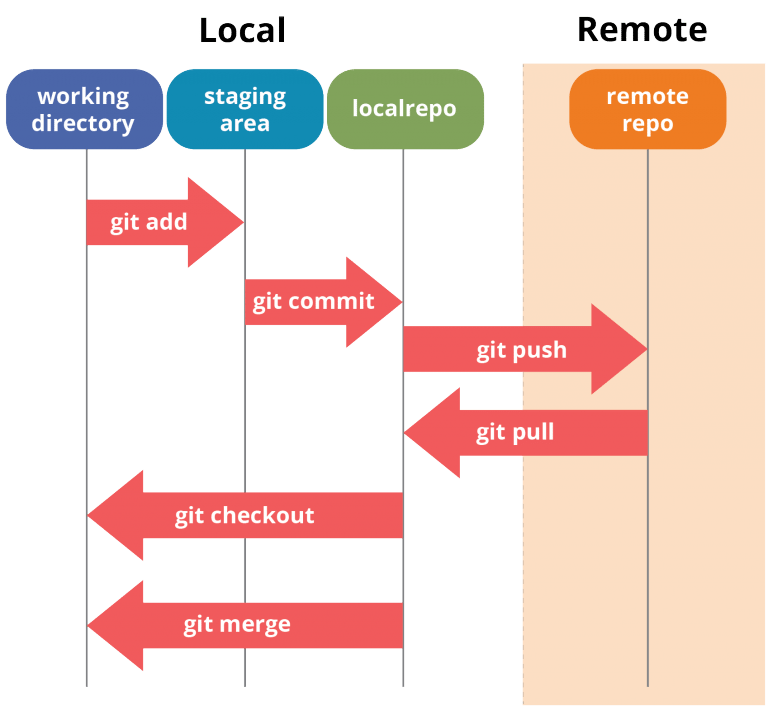
\includegraphics[width=.9\linewidth]{./git.png}
\end{center}

\newpage
\subsection{How to use git?}
\label{sec:orge30e6c6}


\url{https://git-scm.com/downloads/guis}

\begin{center}
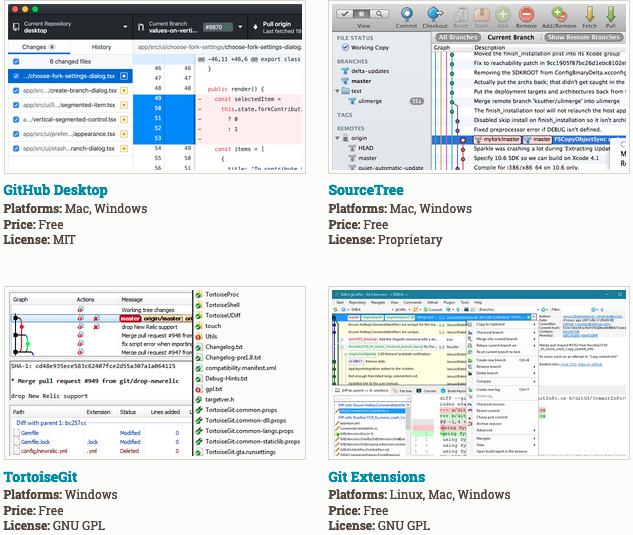
\includegraphics[height=12em]{./s1.png}
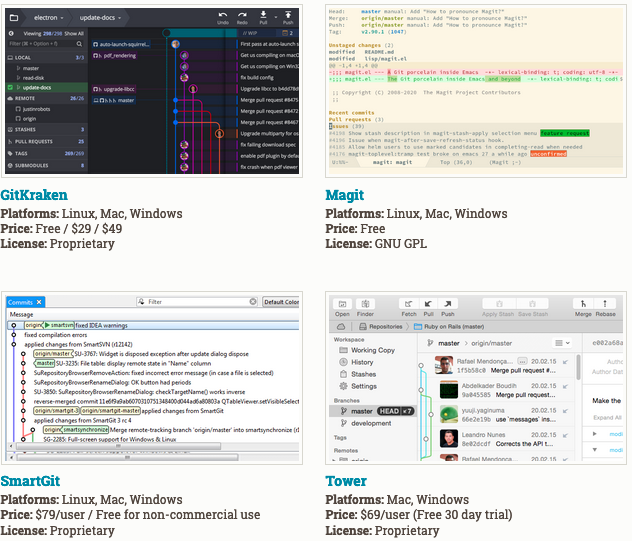
\includegraphics[height=12em]{./s2.png}

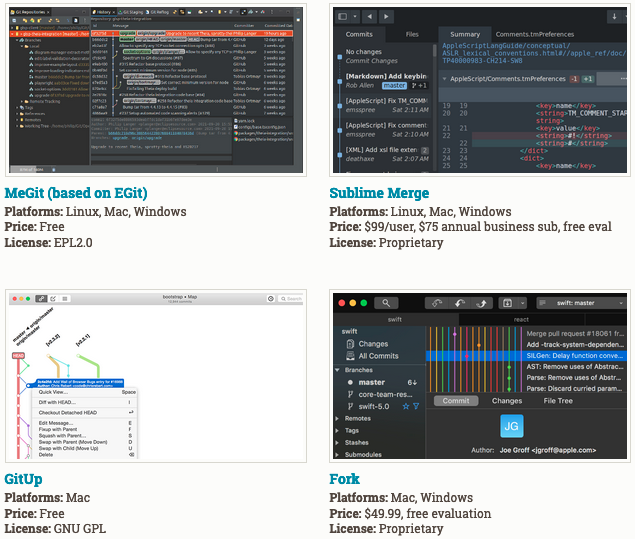
\includegraphics[height=12em]{./s3.png}
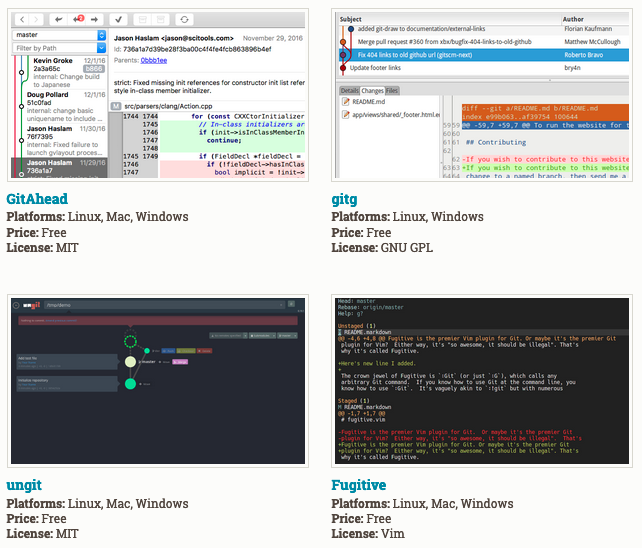
\includegraphics[height=12em]{./s4.png}
\end{center}

\section{Magit}
\label{sec:org650610a}

\begin{center}
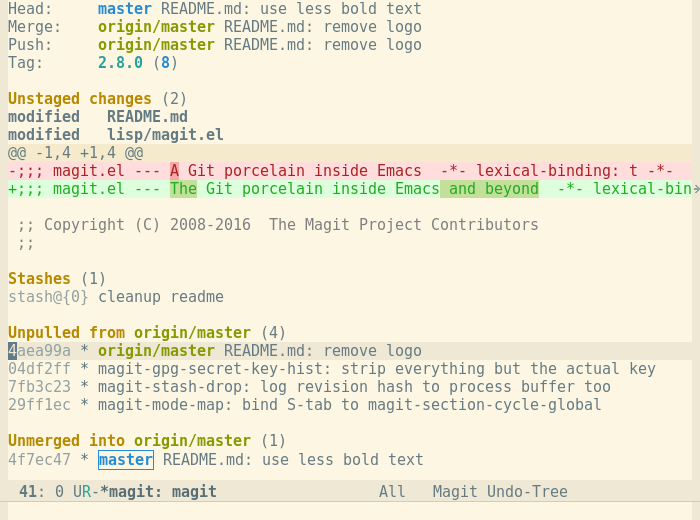
\includegraphics[width=.9\linewidth]{./magit.png}
\end{center}


\subsection{Preparation}
\label{sec:orgec5840e}

\begin{itemize}
\item[{$\square$}] In \texttt{config.el}
\end{itemize}
\begin{verbatim}
;;;; Email information
(setq user-full-name "Maikol Solís"
      user-mail-address "maikol.solis@ucr.ac.cr")
\end{verbatim}

\begin{itemize}
\item[{$\square$}] In \texttt{init.el}
\end{itemize}
\begin{verbatim}
:editor
(evil
 +everywhere)

:tools
(magit
 +forge)
\end{verbatim}

\begin{itemize}
\item[{$\square$}] Create a github repository
\item[{$\square$}] Do example with latex file
\item[{$\square$}] Do example with \texttt{org-roam}
\begin{verbatim}
(after! org-roam
  (setq org-roam-directory
        (file-truename "~/documents/2022/2022_01_Taller_Emacs/roam")))
\end{verbatim}
\end{itemize}

\begin{verbatim}
/Users/maikol/Dropbox/home/documents/2022/2022_01_Taller_Emacs/roam
\end{verbatim}


\begin{itemize}
\item[{$\square$}] Activate \texttt{real-auto-save-mode}
\begin{itemize}
\item In \texttt{packages.el}
\begin{verbatim}
  (package! real-auto-save)
\end{verbatim}
\item In \texttt{config.el}
\begin{verbatim}
   ;;; real-auto-save
   (use-package! real-auto-save
     :hook ((LaTeX-mode . real-auto-save-mode)
            (org-mode . real-auto-save-mode)
            (markdown-mode . real-auto-save-mode)))
\end{verbatim}
\end{itemize}

\item[{$\square$}] Activate \texttt{git-auto-commit-mode}
\begin{itemize}
\item In \texttt{packages.el}
\begin{verbatim}
  (package! git-auto-commit-mode)
\end{verbatim}
\item In \texttt{config.el}
\begin{verbatim}
  (use-package! git-auto-commit-mode
  :config
  (setq gac-automatically-push-p t))
\end{verbatim}
\end{itemize}
\item[{$\square$}] Add \texttt{.dir-locals}
\begin{verbatim}
  ((nil . ((eval git-auto-commit-mode 1)
           (eval real-auto-save-mode 1))))
\end{verbatim}
\end{itemize}
\end{document}